%!TEX TS-program = xelatex
\documentclass[]{friggeri-cv}

\usepackage{afterpage}
\usepackage{hyperref}
\usepackage{color}
\usepackage{xcolor}
\usepackage{wrapfig}
\usepackage{subcaption}
\usepackage{ragged2e}
\usepackage[many]{tcolorbox}
\usepackage{booktabs}
\usepackage[table]{colortbl}
\usepackage{float}
\restylefloat{table}

\hypersetup{
    pdftitle={},
    pdfauthor={},
    pdfsubject={},
    pdfkeywords={},
    colorlinks=false,       % no lik border color
   allbordercolors=white    % white border color for all
}
\addbibresource{bibliography.bib}
\RequirePackage{xcolor}
\definecolor{pblue}{HTML}{0395DE}

\newtcolorbox{aboutmebox}[1][]{
  enhanced,drop fuzzy midday shadow,
  boxrule=1pt,arc=4pt,boxsep=0pt,
  left=1.3em,right=1.3em,top=1.5ex,bottom=1ex,
  colback=blue!15!white,colframe=blue!55!black,#1
}


\begin{document}
\header{Tsvetan}{Dimitrov}
      {Software Developer}
      
% Fake text to add separator      
\fcolorbox{white}{gray}{\parbox{\dimexpr\textwidth-2\fboxsep-2\fboxrule}{%
.....
}}

% In the aside, each new line forces a line break
    
\begin{aside}
    ~
    
\includegraphics[scale=0.11]{img/my_pic_circle.png}
    ~
    
\includegraphics[scale=0.05]{img/github_logo.png}
    \href{https://github.com/powerslider}{github.com/powerslider}
    
\includegraphics[scale=0.1]{img/email_icon.jpg}
    \href{mailto:tsvetan.dimitrov23@gmail.com}{\textbf{tsvetan.dimitrov23@}\\gmail.com}
    
\includegraphics[scale=0.08]{img/skype_logo.png}
    powerslider94
    
\includegraphics[scale=0.08]{img/phone_logo.png}
    +359 88 5131618
    ~
    \begin{aboutmebox}
         I love programming and am a passionate software developer who is very open minded and curious. Although wanting to be a generalist I truly believe that being a specialist in multiple areas brings way more value to the table. My interests are in distributed systems, exploiting new technologies, data visualisation, different programming languages, artificial intelligence. Oh, and I freakin' love Linux!
    \end{aboutmebox}
    ~
    \section{Languages}
    \textbf{English}
\includegraphics[scale=0.40]{img/5stars.png}
    \textbf{German}
\includegraphics[scale=0.40]{img/4stars.png}
    ~
\end{aside}

\section{Programming Skills}
\begin{figure}[h!]  
    \begin{subfigure}[b]{0.4\textwidth}
         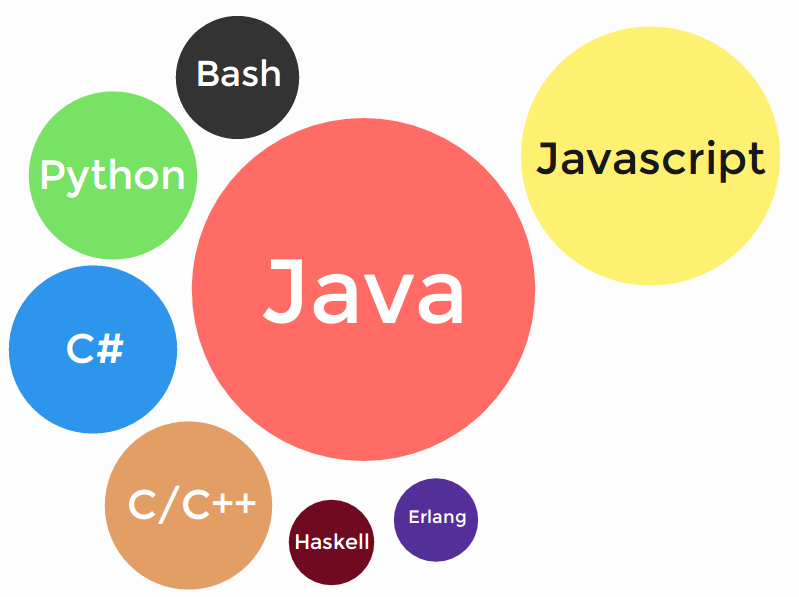
\includegraphics[scale=0.15]{img/programming_language_skills.png}
    \end{subfigure}
    \begin{subfigure}[b]{0.6\textwidth}
        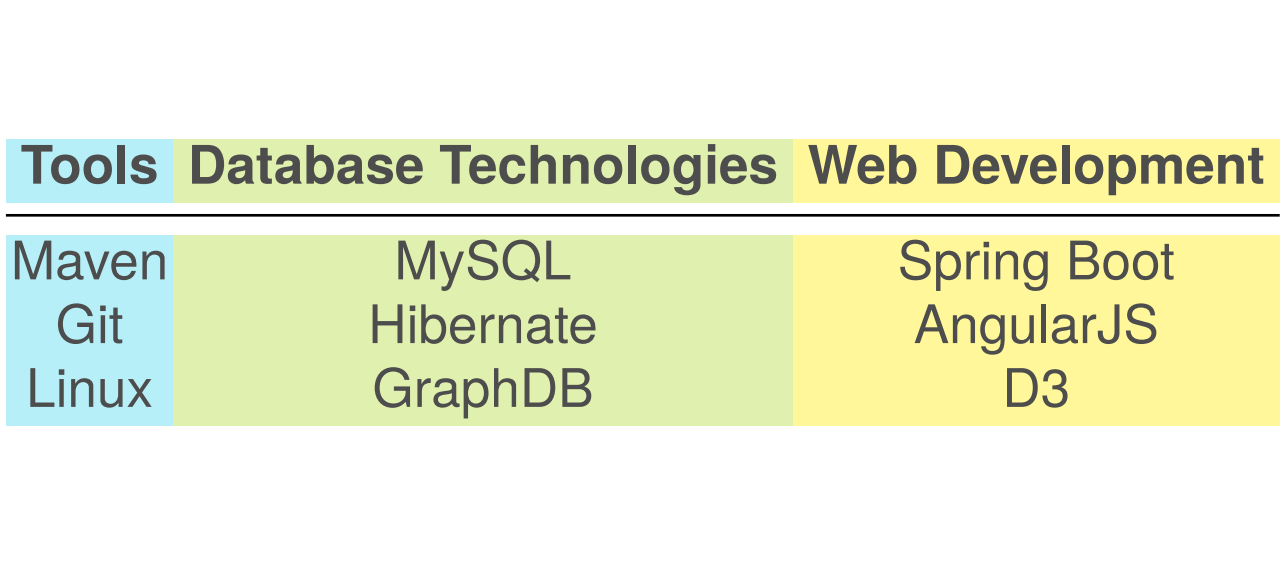
\includegraphics[scale=0.15]{img/programming_technologies.png}
        % \centering
        % \begin{tabular}{c c c}
        %     \cellcolor{blue!50}\textbf{  Tools  } & \cellcolor{green!50}\textbf{  Database Technologies  } & \cellcolor{yellow!50}\textbf{  Web Development  } \\
    
        %     \midrule
        %     \cellcolor{blue!50}Maven & \cellcolor{green!50}MySQL & \cellcolor{yellow!50}Spring Boot\\
        %     \cellcolor{blue!50}Git & \cellcolor{green!50}Hibernate & \cellcolor{yellow!50}AngularJS\\
        %     \cellcolor{blue!50}Linux & \cellcolor{green!50}GraphDB & \cellcolor{yellow!50}D3\\
        % \end{tabular}
    \end{subfigure}
\end{figure}

\section{Experience}
\begin{entrylist}
  \entry
    {03/15 - Now}
    {Software Developer}
    {\textit{Ontotext AD}, Sofia, Bulgaria}
    {Develop external plugins and a workbench for Ontotext's main product GraphDB\textsuperscript{TM} triplestore - a database for semantic metadata. Developed expertise with semantic technologies (RDF, SPARQL), graph databases and visualisation of RDF data.\\}
   \entry
    {05/13 - 03/15}
    {Junior Software Developer}
    {\textit{Ontotext AD}, Sofia, Bulgaria}
    {Responsible for writing / supporting scrapers (crawling agents) for websites in the recruiting sector. Administered the MySQL database of all job vacancies. Developed expertise in many web technologies by using different parsers and transport protocols. }
\end{entrylist}

\section{Certifications}
\begin{entrylist}
    \entry
    {2013}
    {Machine Learning}
    {
\includegraphics[scale=0.4]{img/coursera_logo.png}}
    {Learn basics by completing \texttt{Octave} assignments.}
    
    \entry
    {2014}
    {Web Application Architectures}
    {
\includegraphics[scale=0.4]{img/coursera_logo.png}}
    {Completed a \texttt{Ruby on Rails} webapp.}
    
    \entry
    {2015}
    {Android Basics Course}
    {
\includegraphics[scale=0.1]{img/samsung_logo.png}
\includegraphics[scale=0.1]{img/job_tiger_logo.png}}

    \entry
    {2012}
    {DSD II (Deutsches Sprachdiplom Stufe II)}
    {
\includegraphics[scale=0.2]{img/kmk_logo.png}}
    {German Language certificate level II. Acquired C1 level in all language components.}
\end{entrylist}

\section{Education}
\begin{entrylist}
    \entry
    {2012 - 2016}
    {Bachelor's Degree in Computer Systems\\ and Technologies (in German)}
    {Technical University Sofia}
    {Collaborative undergraduate program w/ Otto-von-Guericke-Universität Magdeburg, Germany.\\
    \emph{\texttt{Thesis:} "Integration of semantic technologies in the processing of news".}}
    
    \entry
    {2015}
    {}
    {Otto-von-Guericke-Universität Magdeburg}
    {Studied 6th semester in \textit{Magdeburg, Germany} in their Informatics undergraduate program, part of my studies @ TU Sofia. Goal is to achieve a double graduation. }
    
    \entry
    {2007 - 2012}
    {}
    {Foreign Language School “Nikola Vapcarov”, Shumen, Bulgaria}
    {\texttt{Main subjects:} German, English, Mathematics.}
\end{entrylist}
\end{document}
